% !TEX root = Master.texs

Within the scope of Section \ref{ssec:kcc_copulas}, an important aspect needs to be taken into consideration. That is the well known fact that correlation does not imply causation. Therefore, alternative frameworks which enable us to detect causal effects shall be briefly discussed in this Section and serve as possible directions for further research.
\\
To illustrate an application of a dynamic Bayesian network (\ac{DBN}, see Section \ref{ssec:bayesian_networks}) with the help of the R package \textit{dbnR}, which is an implementation of Gaussian dynamic Bayesian networks (GDBN) structure learning and inference based on Marco Scutari’s package \textit{bnlearn} \citep{bnlearn_package}, we delimit ourselves to key category cluster 1 since it contains only 14 distinct articles (see \autoref{tab:articles_in_kcc_1}) and assures clear (graphical) overview. 
For details on the implementation of the structure learning algorithm, one can refer to the documentation of the \textit{dbnR} package.
\\

\begin{table}[H]
\setlength\arrayrulewidth{1pt}  
\centering
\begin{adjustbox}{max width=\textwidth}\
\begin{tabular}{|c|c|c|c|c|c|c|c|c|c|c|c|c|c|}
\hline
10327 & 10328 & 13450 & 13451 & 19 & 19137 & 19138 & 21 & 24558 & 26191 & 26192 & 26193 & 26194 & 615 \\ \hline
\end{tabular}
\end{adjustbox}
\caption{Articles in key category cluster 1}
\label{tab:articles_in_kcc_1}
\end{table}








\begin{figure}[H]
\centering
  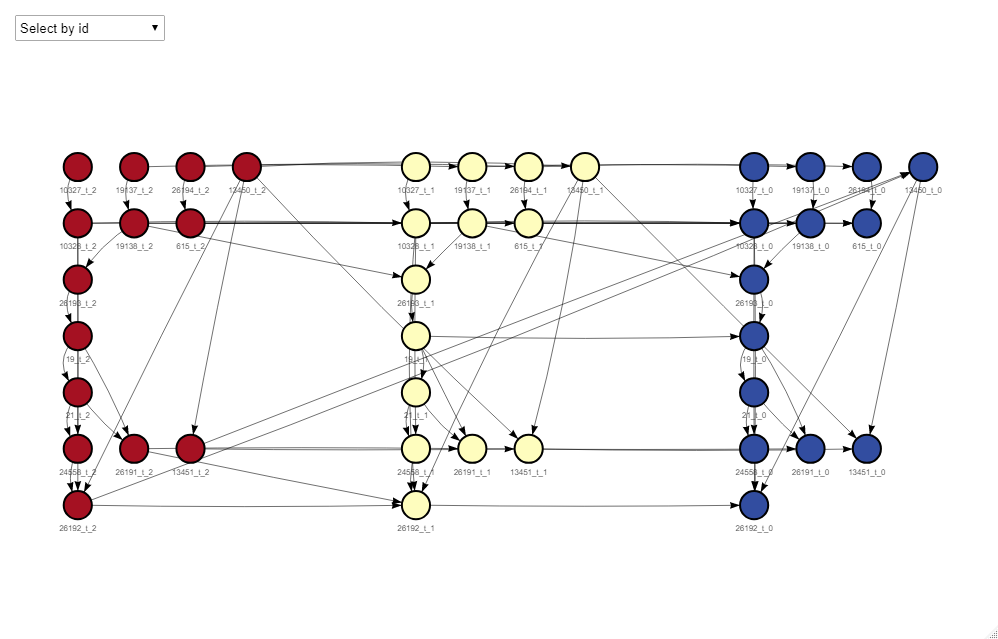
\includegraphics[width=0.85\linewidth]{figures/dbn_kcc_1_all.png}
  \caption{Graphical representation of the dynamic Bayesian network for articles in key category cluster 1 - The blue nodes indicate articles at the current time-point $t_0$, the yellow nodes indicate the same articles at one previous time point $t_1$ and the red nodes indicate the articles at two previous time points $t_2$}
  \label{fig:dbn_kcc_1_all}
\end{figure}




\begin{figure}[H]
\centering
  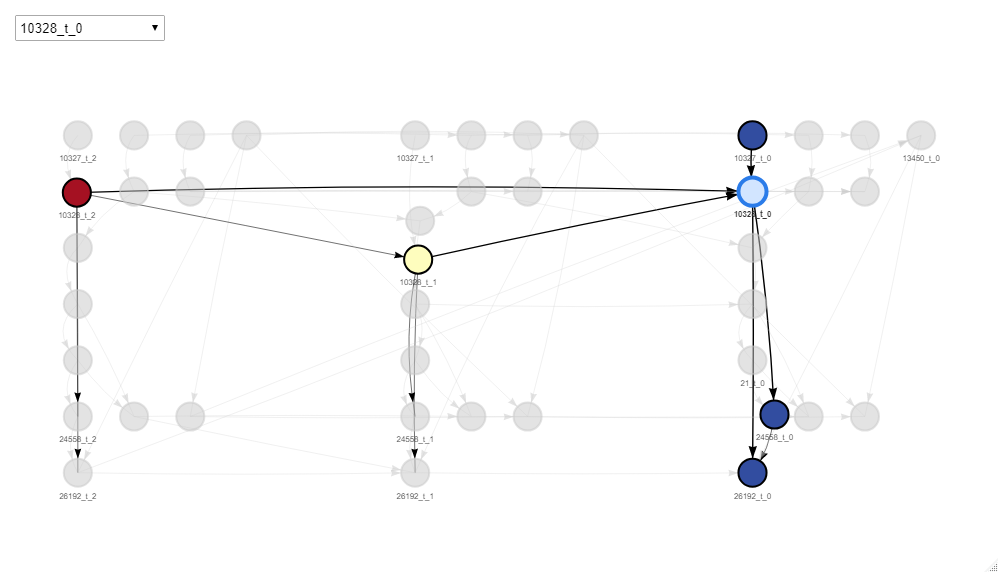
\includegraphics[width=0.85\linewidth]{figures/dbn_kcc_1_article_10328_t_0.png}
  \caption{Dynamic Bayesian network graph of KCC 1 highlighting article \textit{"10328"} at latest time-point $t_0$ and all of its adjacent nodes}
  \label{fig:dbn_kcc_1_article_10328_t_0}
\end{figure}



The \textit{dbnR} package allows Markovian orders higher than 1, i.e. \ac{VAR}($p$) processes with $p \geq 1$, and an optional setting for forbidding arcs between nodes. For this exercise, such constraints are dismissed and the structure of a Markovian \ac{DBN} of order 2 is learned by the algorithm. A summary of the net's structure can be found in the Appendix (R output \ref{output:dbnR_output_kcc_1}). Note that the latest (current) time-point is denoted by $t_0$ in this context, so $t_1$ is one lag and $t_2$ are two lags. The example depicted in \ref{fig:dbn_kcc_1_all} shows how any node can be the cause of another node at the same or a later time-point, but not for a past time-point. \\
 Graphical representations are depicted in Figures \ref{fig:dbn_kcc_1_all} and \ref{fig:dbn_kcc_1_article_10328_t_0}, the latter highlighting the node of article with ID \textit{"10328"} at time-point $t_0$ (highlighted blue node) and all of its adjacent nodes.